
\subsection{Method and Implementation}

Once the channel images have been generated by using the received channel measurements as described in Section \ref{image-gen}, the spots or 'stars' within the images need to be located for channel reconstruction. This is done using the fast object detection model YOLO to identify bounding boxes for each of the spots in the images. Before using YOLO to detect the target objects within our channel images, a YOLO model needs to be trained with labelled data, so the Darknet-53 learning model can adapt to a new application. This type of learning is called transfer learning as a previously trained network is used and re-trained at a lower cost than training a network with fresh weights \cite{Burkov2019}.

Before we can train our object detection model, a training, validation, and test set of labelled data need to be generated. Many images can be generated using the image generation technique discussed in Section \ref{image-gen}, but to label the images require manual assignment of bounding boxes around the spots in the channel images. This process can be very slow, especially if the number of paths/spots or noise in the image is high. To label the bounding boxes of the spots in the image, MATLAB's Image Labeler was used to manually draw the bounding boxes for several hundred images. These images and their ground truth data are provided to the YOLO training algorithm in MATLAB to produce a detector of the white spots in the grayscale images produced by the image generator.

YOLO's network structure is described in YOLO subsection in Section \ref{background}. The image input size for the input layer of the neural network is $256 \times 256$ pixels with three colour channels. The images generated for channel estimation in Section \ref{image-gen} are $1536 \times 1536$ grayscale images which mean that the images only contain one colour channel and do not meet the requirements for the input layer of YOLO. Therefore, before the training images and bounding boxes are inserted into the trainer, the training and validation images need to be preprocessed to transform their size to the input size and add two more colour channels for full RGB capability. The preprocessing of the images used for training and validation occur before executing the training process. After training has completed, images that would like to be searched by the detector model will have to reformat themselves, as in the preprocessing steps, to extract the target objects from the images and meet the network's input requirements. As for the middle hidden layers, YOLOv3 uses the Darknet-53 network model for object detection. As our detection objects are quite simple, black background with white spots, all 53 convolution layers are not needed to preform the object detection to an acceptable degree. The convolution layer depth of the network can be set as a hyperparameter and modified in an attempt to produce a detector with the highest precision. In the case of this project, after training multiple different layer length neural networks, it was determined that the weighted Darknet-53 network would produce sufficient results when using up to the $33^{rd}$ convolution layer. The layers after that point are removed and replaced with the final transform and output layers. The transform and output layers are attached to the end of the network at the convolution layer 33 and convert the values from the network to functional predictions of the locations of spots within the channel image.

Now that the labelled training data has been collected and the network structure has been finalized, the training of the DNN can begin. The training options specified in MATLAB's training algorithms can be varied depending on the application. For the following project the YOLO network was trained on a Nvidia GTX 1060 3GB which has a small amount of VRAM and therefore cannot process large amounts of data in the Mini-batches of the Stochastic Gradient Descent with Momentum (SDGM) training technique for deep neural networks \cite{Burkov2019, Matlab2021a}. Due to the aforementioned resource restriction in VRAM, the Mini-batch size was set to 6. A maximum of 20 epochs are used during training to set a reasonable end to training a pre-trained network.

\subsection{Results}

\begin{figure}[H]
\centering
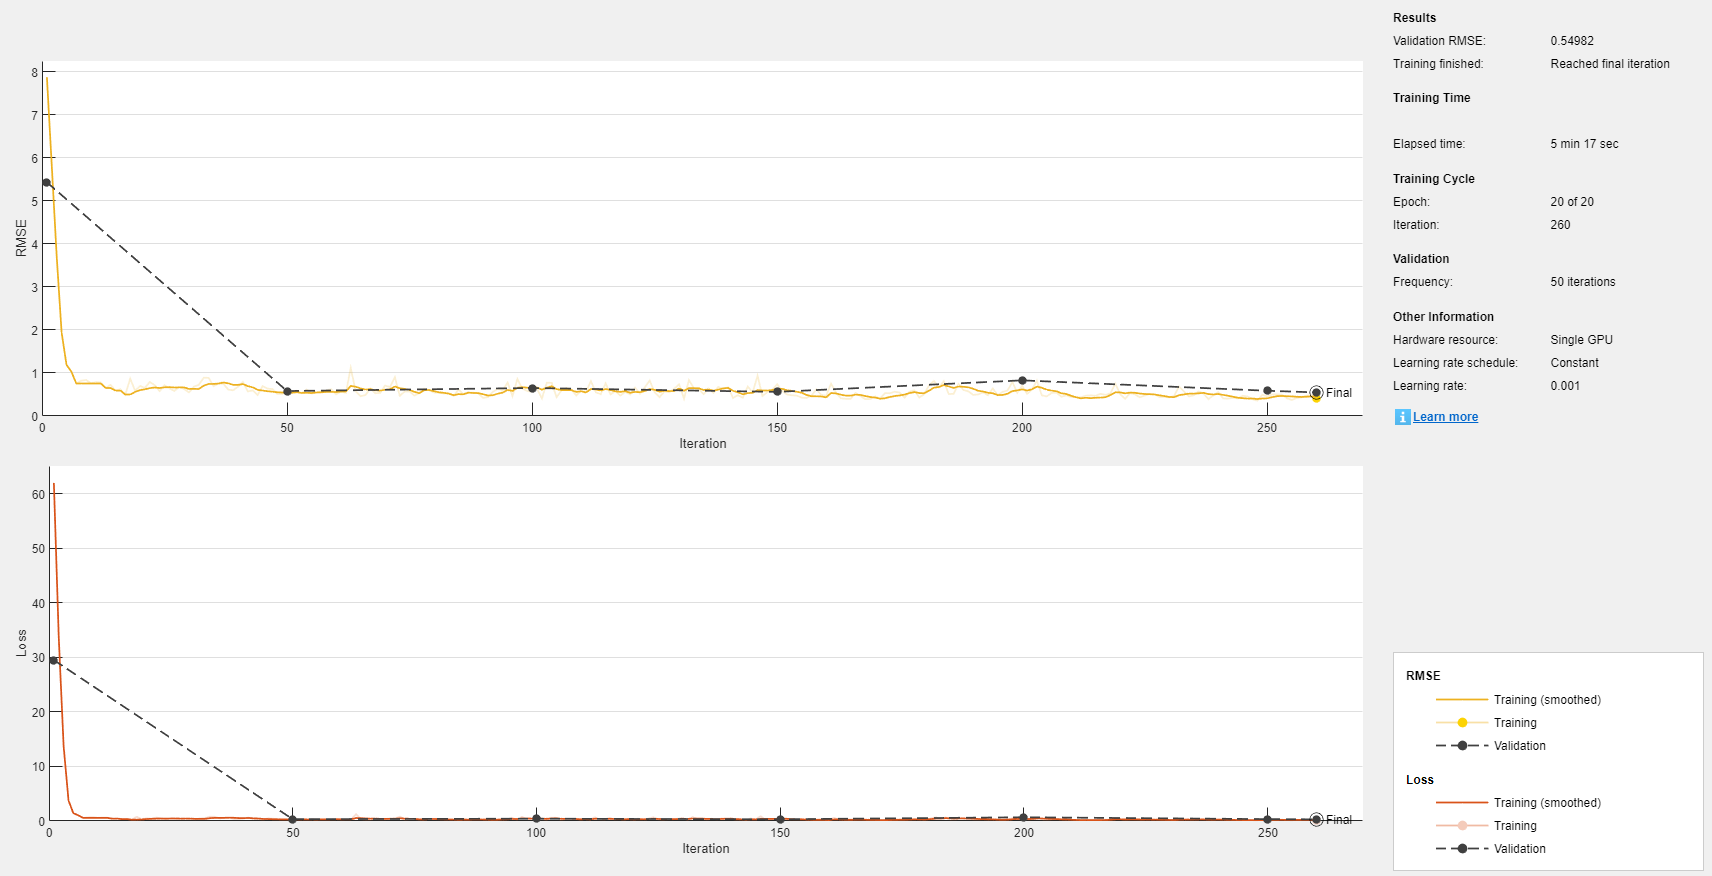
\includegraphics[width=0.9\textwidth]{figures/YOLOv3-training-2-weights-conv30.PNG}
\caption{The progression of training the YOLO model using SGDM}
\label{fig:yolo-training}
\end{figure}

Figure \ref{fig:yolo-training} shows the training progress of one of the trained detectors for the project. The top chart shows the Root Mean Squared Error (RMSE) of the model over each Mini-batch iteration with the dotted line representing the RMSE for the validation dataset. The bottom chart shows the loss over each of the iteration during training with the dotted line representing the loss of the validation set every 50 iterations. The two charts form the classic elbow shape of machine learning models using SGDM for their training as it quickly falls into a local minimum and then searches for further minimums in subsequent iterations with marginal changes. The training progress charts are updated live with the training progress in MATLAB and are very handy in monitoring and debugging the network and tuning the hyperparameters of the model.

\begin{figure}[H]
    \subfigure[]{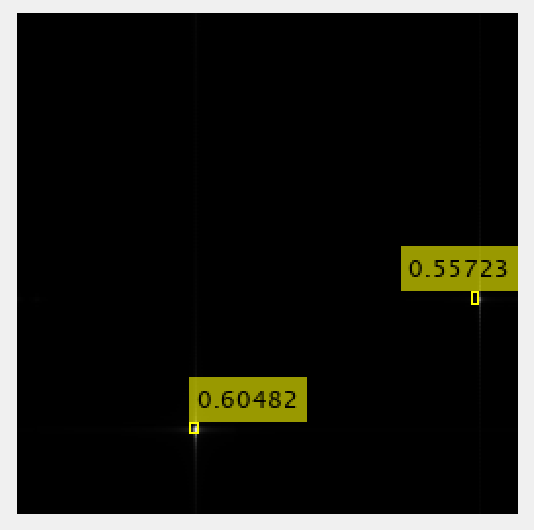
\includegraphics[width=0.3\textwidth]{CaptureExample2.PNG}}
    \subfigure[]{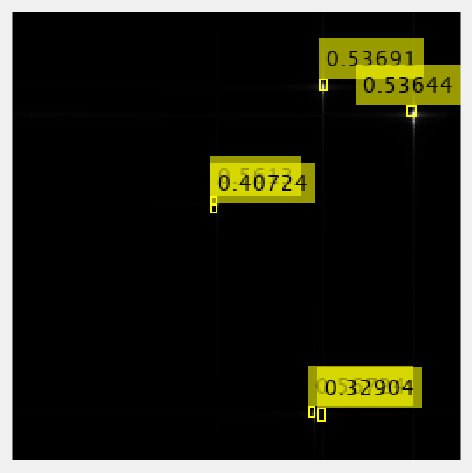
\includegraphics[width=0.3\textwidth]{CaptureExample.PNG}}
    \subfigure[]{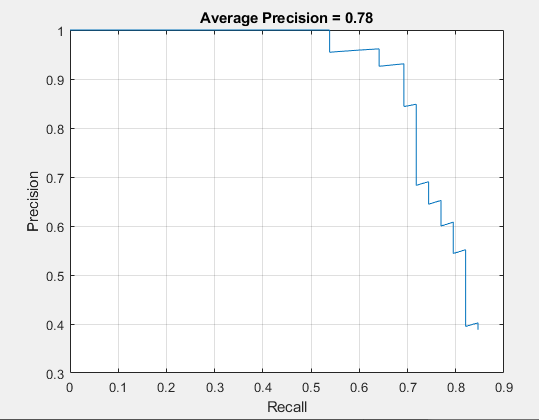
\includegraphics[width=0.38\textwidth]{YOLOv3-PRC-threshold0-25-conv30.PNG}} 
    \caption{Examples of object detection using the trained YOLO model}
    \label{fig:yolo}
\end{figure}

After the YOLO object detection model has been trained using the labelled data, testing data can be used to predict the average precision and generate plots such as the Precision-Recall Curve to evaluate the precision and recall of our detector. The Precision-Recall Curve can then be used to tune the threshold of the detector. In figure \ref{fig:yolo}c, the threshold is set to 0.25, where the threshold represents the probability that a prediction must be greater than or equal to, to be considered as a target object and returned in the detection of the model. The Precision-Recall Curve is used to evaluate the positive rate of the minority class \cite{Burkov2019}. In channel reconstruction it is important for the precision to be high, so the detector does not find false paths in the channel matrix. The recall should also be high so paths are not missed in detection. Balancing these two metrics can be difficult when tuning the machine learning model, but the Precision-Recall Curve aid in a understanding of how the model moves with respect to changes of the hyperparameters, such as threshold.

Figure \ref{fig:yolo} (a) and (b) provide examples of the detection of spots or paths within the channel image. A lower threshold is used so that fainter path components can be picked up by the detector, but many of the detected spots are detected without difficulty.

\subsection{Discussion}

Our project uses Matlab's 2021a Computer Vision, Deep Learning, and Image Processing modules which supposedly include a YOLOv2 and YOLOv3 implementation and their backing networks (Darknet-19 and Darknet-53) \cite{Matlab2021a,Matlab2021b}. During the implementation of YOLO in our project the work from \cite{Li2020,Matlab2021a,Matlab2021b} were used to construct the defined YOLOv3 for the path detection in the generated channel images. To our surprise, although the documentation was available for the YOLOv3 network, the actual network and appropriate functions defined in the documentation were not available in the latest release of MATLAB (2021a). YOLOv3's Darknet-53 network structure is available in MATLAB's deep network designer and could be installed separately to the other deep learning functions in the Deep Learning Module. Therefore, previous YOLOv2 input, transform, and output layers could be used with the Darknet-53 structure to create the YOLOv3 network without the functions described in \cite{Matlab2021b}.

When initially labelling the spots in the images for object detection, the authors drew the bounding boxes too small around the spots. This lead to a difficulty of predicting the bounding boxes for unlabelled data. This is believed to be so since the images are preprocessed and shrunk to fit the image size requirements of the input layer of the YOLO network. Small labelled bounding boxes would be transformed into small boxes with little area within and thus making the learning process for the detector more challenging. To overcome this issue, the authors were more relaxed on the bounds of the boxes around the spots in the image and the precision of the model saw a large jump.

To improve the precision of the object detection model, more labelled data should be generated. This would increase available labelled data for the training of current and future deep learning methods that use the channel image for path extraction and channel reconstruction. Most of the labelled data also contains little to no noise at all in the image, so the current detector performs poorly when attempting to identify spots in a noisy channel. This can't be the case in an actual m-MIMO system because the noise levels vary over time and space and must be accounted for in the machine learning model.